\documentclass[landscape,twocolumn,letterpaper,9pt,reqno]{article}\usepackage[]{graphicx}\usepackage[]{color}
%% maxwidth is the original width if it is less than linewidth
%% otherwise use linewidth (to make sure the graphics do not exceed the margin)
\makeatletter
\def\maxwidth{ %
  \ifdim\Gin@nat@width>\linewidth
    \linewidth
  \else
    \Gin@nat@width
  \fi
}
\makeatother

\definecolor{fgcolor}{rgb}{0.345, 0.345, 0.345}
\newcommand{\hlnum}[1]{\textcolor[rgb]{0.686,0.059,0.569}{#1}}%
\newcommand{\hlstr}[1]{\textcolor[rgb]{0.192,0.494,0.8}{#1}}%
\newcommand{\hlcom}[1]{\textcolor[rgb]{0.678,0.584,0.686}{\textit{#1}}}%
\newcommand{\hlopt}[1]{\textcolor[rgb]{0,0,0}{#1}}%
\newcommand{\hlstd}[1]{\textcolor[rgb]{0.345,0.345,0.345}{#1}}%
\newcommand{\hlkwa}[1]{\textcolor[rgb]{0.161,0.373,0.58}{\textbf{#1}}}%
\newcommand{\hlkwb}[1]{\textcolor[rgb]{0.69,0.353,0.396}{#1}}%
\newcommand{\hlkwc}[1]{\textcolor[rgb]{0.333,0.667,0.333}{#1}}%
\newcommand{\hlkwd}[1]{\textcolor[rgb]{0.737,0.353,0.396}{\textbf{#1}}}%
\let\hlipl\hlkwb

\usepackage{framed}
\makeatletter
\newenvironment{kframe}{%
 \def\at@end@of@kframe{}%
 \ifinner\ifhmode%
  \def\at@end@of@kframe{\end{minipage}}%
  \begin{minipage}{\columnwidth}%
 \fi\fi%
 \def\FrameCommand##1{\hskip\@totalleftmargin \hskip-\fboxsep
 \colorbox{shadecolor}{##1}\hskip-\fboxsep
     % There is no \\@totalrightmargin, so:
     \hskip-\linewidth \hskip-\@totalleftmargin \hskip\columnwidth}%
 \MakeFramed {\advance\hsize-\width
   \@totalleftmargin\z@ \linewidth\hsize
   \@setminipage}}%
 {\par\unskip\endMakeFramed%
 \at@end@of@kframe}
\makeatother

\definecolor{shadecolor}{rgb}{.97, .97, .97}
\definecolor{messagecolor}{rgb}{0, 0, 0}
\definecolor{warningcolor}{rgb}{1, 0, 1}
\definecolor{errorcolor}{rgb}{1, 0, 0}
\newenvironment{knitrout}{}{} % an empty environment to be redefined in TeX

\usepackage{alltt}

\usepackage{lscape,fancyhdr}

\usepackage{hyperref}

\pagestyle{fancy}

\usepackage{amsmath,epsfig,subfigure,amsthm,amsfonts,epsf,psfrag,rotating,setspace,bm}

\usepackage{verbatim,color} % Allow text colors}

\setlength{\oddsidemargin}{-0.4in}		% default=0in
\setlength\evensidemargin{-0.4in}

\setlength{\textwidth}{9.8in}		% default=9in

\setlength{\columnsep}{0.5in}		% default=10pt

\setlength{\columnseprule}{0pt}		% default=0pt (no line)


\setlength{\textheight}{7.0in}		% default=5.15in

\setlength{\topmargin}{-0.75in}		% default=0.20in

\setlength{\headsep}{0.25in}		% default=0.35in

\setlength{\parskip}{1.2ex}

\setlength{\parindent}{0mm}

\lhead{Course EPIB607: Regression handout 006 (Logistic regression)}
\rhead{jh,sb \ \ \ v. 2018.11.26}
\IfFileExists{upquote.sty}{\usepackage{upquote}}{}
\begin{document}
	


\section{Cesarean section and transmission of HIV}

\begin{figure}[h]
	\centering
	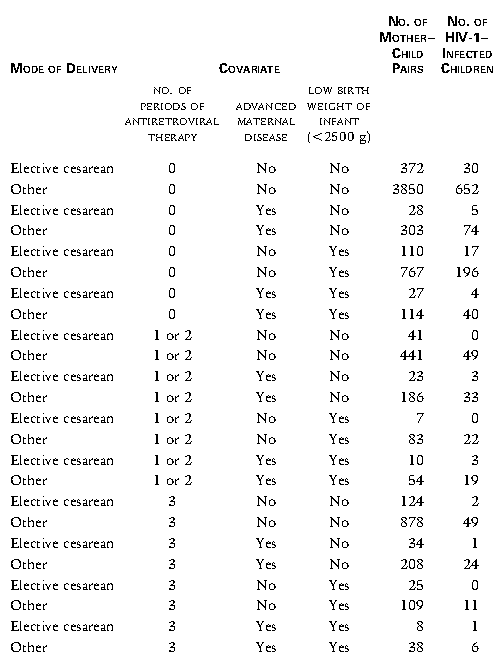
\includegraphics[scale=0.99]{hivtable.pdf}
\end{figure}


\begin{knitrout}
\definecolor{shadecolor}{rgb}{0.969, 0.969, 0.969}\color{fgcolor}
\begin{verbatim}
## 
## Call:
## glm(formula = cbind(cases, controls) ~ open, family = binomial(link = "logit"), 
##     data = df)
## 
## Deviance Residuals: 
## [1]  0  0
## 
## Coefficients:
##             Estimate Std. Error z value Pr(>|z|)    
## (Intercept)  -1.5556     0.1409 -11.040   <2e-16 ***
## open          0.2899     0.1911   1.517    0.129    
## ---
## Signif. codes:  0 '***' 0.001 '**' 0.01 '*' 0.05 '.' 0.1 ' ' 1
## 
## (Dispersion parameter for binomial family taken to be 1)
## 
##     Null deviance: 2.3148e+00  on 1  degrees of freedom
## Residual deviance: 9.9920e-15  on 0  degrees of freedom
## AIC: 15.696
## 
## Number of Fisher Scoring iterations: 3
\end{verbatim}

\end{knitrout}

\clearpage

\section{Smoking among women in Whickham, England}


\begin{table}[h]
	\centering
	\begin{tabular}{lcccc}
		 &  &   \multicolumn{2}{c}{Smoking} &  \\		
		Age & Vital Status &  Yes & No & Total \\
		18-24 	& Dead 	& 2  	& 1 	& 3 	\\	
		 		& Alive & 53  	& 61 	& 114 	\\
		 		& Risk & 0.04  	& 0.02 	& 0.03 	\\
		 		\hline
		25-34 	& Dead 	& 3  	& 5 	& 8 	\\	
& Alive & 121  	& 152 	& 273 	\\
& Risk & 0.02  	& 0.03 	& 0.03 \\
\hline 			
35-44 	& Dead 	& 14  	& 7 	& 21 	\\	
& Alive & 95  	& 114 	& 209 	\\
& Risk & 0.13  	& 0.06 	& 0.09 \\
\hline
45-54 	& Dead 	& 27  	& 12 	& 39 	\\	
& Alive & 103  	& 66 	& 169 	\\
& Risk & 0.21  	& 0.15 	& 0.19 \\
		 		\hline
55-64 	& Dead 	& 51  	& 40 	& 91 	\\	
& Alive & 64  	& 81 	& 145 	\\
& Risk & 0.44  	& 0.33 	& 0.39 \\
		 		\hline
65-74 	& Dead 	& 29  	& 101 	& 130 	\\	
& Alive & 7  	& 28 	& 35 	\\
& Risk & 0.81  	& 0.78 	& 0.79 \\
		 		\hline
75+ 	& Dead 	& 13  	& 64 	& 77 	\\	
& Alive & 0  	& 0 	& 0 	\\
& Risk & 1.00  	& 1.00 	& 1.00 \\
\hline
	\end{tabular}
\end{table}


\begin{knitrout}
\definecolor{shadecolor}{rgb}{0.969, 0.969, 0.969}\color{fgcolor}
\begin{verbatim}
## 
## Call:
## glm(formula = cbind(cases, controls) ~ open + size, family = binomial(link = "logit"), 
##     data = df)
## 
## Deviance Residuals: 
##       1        2        3        4  
## -0.7636   0.3588   0.2756  -0.4695  
## 
## Coefficients:
##             Estimate Std. Error z value Pr(>|z|)    
## (Intercept)  -1.9366     0.1704 -11.361  < 2e-16 ***
## open         -0.3572     0.2291  -1.559    0.119    
## size          1.2606     0.2390   5.274 1.33e-07 ***
## ---
## Signif. codes:  0 '***' 0.001 '**' 0.01 '*' 0.05 '.' 0.1 ' ' 1
## 
## (Dispersion parameter for binomial family taken to be 1)
## 
##     Null deviance: 33.1239  on 3  degrees of freedom
## Residual deviance:  1.0082  on 1  degrees of freedom
## AIC: 26.355
## 
## Number of Fisher Scoring iterations: 3
\end{verbatim}

\end{knitrout}

\clearpage

\section{Diabetes cohort data 1}

\begin{table}[h]
	\centering
	\begin{tabular}{lcc|c}
		& Dead &  Censored & Total\\
		Type II & 218 & 326 & 544 \\
		Type I & 105 & 253 & 323 \\
		\hline
		Total & 323 & 579 & 902
	\end{tabular}
\end{table}


\begin{knitrout}
\definecolor{shadecolor}{rgb}{0.969, 0.969, 0.969}\color{fgcolor}
\begin{verbatim}
## 
## Call:
## glm(formula = cbind(cases, controls) ~ type, family = binomial(link = "logit"), 
##     data = df)
## 
## Deviance Residuals: 
## [1]  0  0
## 
## Coefficients:
##             Estimate Std. Error z value Pr(>|z|)    
## (Intercept)  -0.8794     0.1161  -7.576 3.58e-14 ***
## type          0.4770     0.1454   3.282  0.00103 ** 
## ---
## Signif. codes:  0 '***' 0.001 '**' 0.01 '*' 0.05 '.' 0.1 ' ' 1
## 
## (Dispersion parameter for binomial family taken to be 1)
## 
##     Null deviance: 1.0978e+01  on 1  degrees of freedom
## Residual deviance: 1.4033e-13  on 0  degrees of freedom
## AIC: 16.858
## 
## Number of Fisher Scoring iterations: 2
\end{verbatim}

\end{knitrout}



\clearpage

\section{Diabetes cohort data 2}

Below are the same outcomes tabulated by age:

\begin{table}[h]
	\centering
	\begin{tabular}{lcc|c}
		$\leq 40$ & Dead &  Censored & Total\\
		Type II & 0 & 15 & 15 \\
		Type I & 1 & 129 & 130 \\
		\hline
		Total & 1 & 144 & 145 \\
		& & & \\
		$> 40$ & Dead &  Censored & Total\\
		Type II & 218 & 311 & 529 \\
		Type I & 104 & 124 & 228 \\
				\hline
		Total & 322 & 435 & 757 \\ 
	\end{tabular}
\end{table}


\begin{knitrout}
\definecolor{shadecolor}{rgb}{0.969, 0.969, 0.969}\color{fgcolor}
\begin{verbatim}
## 
## Call:
## glm(formula = cbind(dead, censored) ~ type + age, family = binomial(link = "logit"), 
##     data = df)
## 
## Deviance Residuals: 
##        1         2         3         4  
## -0.41982   0.09091   0.00776  -0.01168  
## 
## Coefficients:
##             Estimate Std. Error z value Pr(>|z|)    
## (Intercept)  -4.9525     1.0036  -4.935 8.02e-07 ***
## type         -0.1816     0.1595  -1.139    0.255    
## age           4.7781     1.0108   4.727 2.28e-06 ***
## ---
## Signif. codes:  0 '***' 0.001 '**' 0.01 '*' 0.05 '.' 0.1 ' ' 1
## 
## (Dispersion parameter for binomial family taken to be 1)
## 
##     Null deviance: 133.81237  on 3  degrees of freedom
## Residual deviance:   0.18471  on 1  degrees of freedom
## AIC: 20.745
## 
## Number of Fisher Scoring iterations: 5
\end{verbatim}

\end{knitrout}



\end{document}
